\subsection{Short term speckle pulsing}

To measure the PSD and the cutoff $k_c$ of speckle potential with short time speckle pulsing, we derive the evolution of the momentum state under two approximations. The first is the Raman-Nath approximation, atoms don’t move far during the pulse.  The second is that the evolution time is short compared to $\hbar/V(x)$, so atoms don’t acquire a phase comparable to $2\pi$.
Consider Hamiltonian
\begin{equation}
    \hat{H} = \frac{\hbar^2k^2}{2m} + V(x).
\end{equation}
The time evolution operator is
\begin{equation}
    \hat{U}(t) = \exp{-i\frac{\Delta t}{\hbar}\left[\frac{\hbar^2k^2}{2m}+V(x)\right]},
\end{equation}
Define $E_c$ as the energy associated with $k_c$, $\tau = \frac{\Delta t}{\hbar}E_c$, $\hat{k} = \frac{k}{k_c}$ and $S(x) = \frac{V(x)}{E_c}$
\begin{equation}
    \hat{U}(t) = \exp{-i\tau\left[\hat{k}^2+S(x)\right]}.
\end{equation}
Expand the operator to second order, 
\begin{equation}
    \hat{U}(t) = \exp{-i\tau\hat{k}^2/2}\exp{-i\tau S(x)}\exp{-i\tau\hat{k}^2/2}.
\end{equation}
We assume the initial state is $\ket{k=0}$ so the third term does not contribute, and we measure the distribution is $k$ space, so we can ignore the first term. The second term governs the short time evolution. To lowest order, 
\begin{equation}
    \hat{U}(t)\ket{k=0} = \ket{k=0} - i\tau S(x) \ket{k=0}
\end{equation}
Expand $S(x)$ in $k$ space,
\begin{equation}
    S(x) = \sum_{k,k'}\Tilde{S}(k-k')\dyad{k}{k'}
\end{equation}
So
\begin{equation}
    \hat{U}(t)\ket{k=0} = \ket{k=0} - i\tau \sum_{\delta k}\Tilde{S}(\delta k)\ket{\delta k}
\end{equation}
The state probability distribution at time $\tau$ is
\begin{equation}
    P(k,\tau) = \tau^2 |\Tilde{S}(\delta k)|^2 + \delta_{k,0}
\end{equation}
proportional to the PSD $|\Tilde{S}(\delta k)|^2$.

In the experiment, we put a iris right before the diffuser $D$ in \ref{fig:design}. Bu opening and closing the iris, we can control the size of the beam which determines $k_c$ of the speckle potential PSD in the focal plane. As the model we derived in \ref{speckle_chapter} shows, the speckle beam size at the focal plane does not change when the beam size at the diffuser changes. The beam size at the focal plane is determined by the field-field correlation length at the the diffuser. So the average speckle potential depth is proportional to the power of the beam which we can measure with a photodiode(PD). 

Our experimental sequence start with a BEC held in a cross dipole trap. Immediately after turning off the dipole trap, we pulse the speckle beam for time $\tau$, followed by a time-of-flight (TOF). An absorption image is taken after the TOF. For the data we took, $\tau$ range from $0 {\rm ms}$ to $6 {\rm ms}$. The TOF maps the momentum distribution to the position distribution. So by analysing the optical depth of the images, we can get the momentum distribution of atoms after the speckle pulsing and compute its width from which, the average kinetic energy and average speckle potential depth can be estimated.

\begin{figure*}
    \centering
    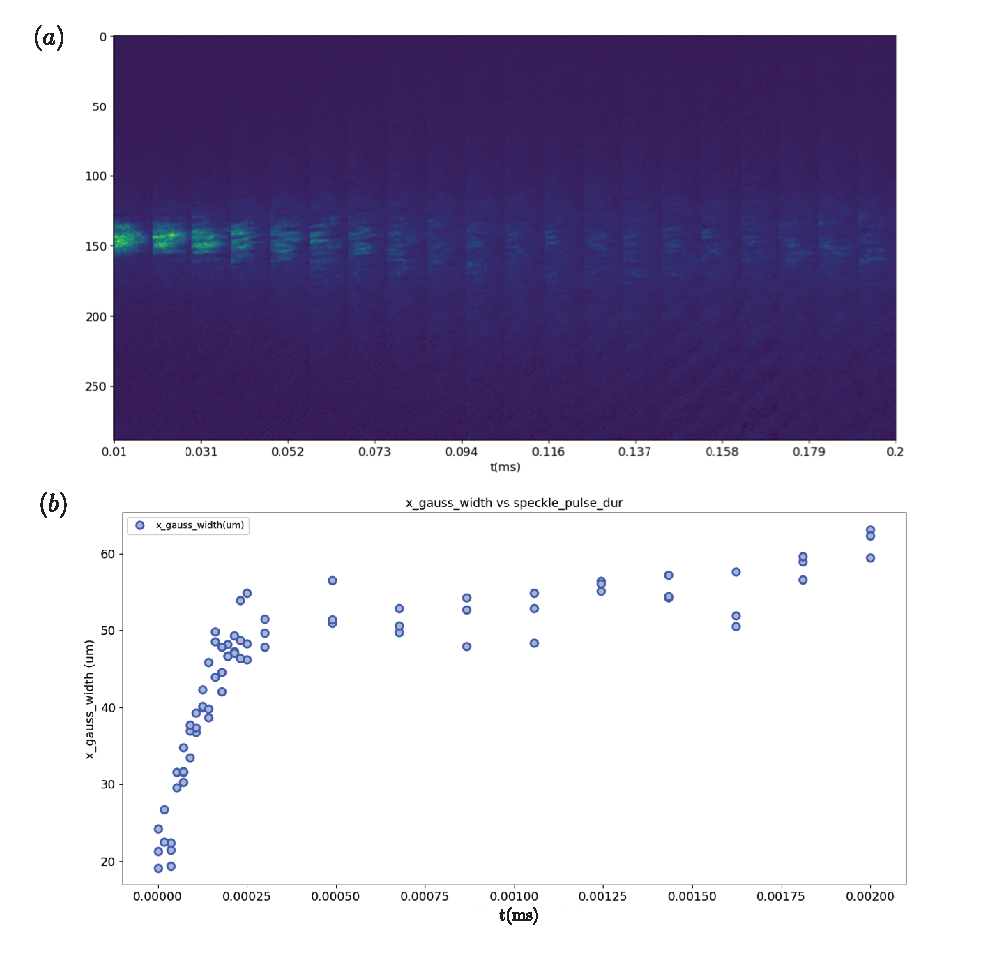
\includegraphics{Chapter6_secs/speckle_pulsing_data.pdf}
    \caption{Speckle beam pulsing data. (a). Absorption images after TOF for different speckle pulsing time. The width of atoms increases as the speckle pulsing time increases from 0 to $\approx 2 {\rm ms}$. After which the width reaches equilibrium. (b). The Gaussian width of atoms in absorption images for  different speckle pulsing time.}
    \label{fig:speckle_pulsing}
\end{figure*}

Fig.~(\ref{fig:speckle_pulsing}) shows absorption images and the fitted Gaussian width. With TOF, the momentum distribution of atoms after speckle pulsing is mapped to the distribution in space. So the optical depth of the absorption images is proportional to the momentum distribution before TOF. For short time speckle pulsing, the width of the momentum distribution increases rapidly. After $\approx 2 {\rm ms}$, the atoms reach equilibrium under speckle potential and the width of the momentum distribution reaches maximum. The average kinetic energy of the atoms can be calculated from the width of momentum distribution in equilibrium. And by Virial Theorem, the total energy can be calculated and compared with the average speckle potential depth. As Fig.~(\ref{fig:speckle_pulsing})(a) shows, we measure the photodiode reading which is proportional to the power of the speckle beam and the average speckle depth. We fit a line crossing the origin so the average speckle potential can be inferred by the photodiode reading directly.

As our model shows, in short time speckle pulsing, the momentum distribution should be proportional to the speckle potential PSD except for the peak at $k=0$. In Fig.~(\ref{fig:speckle_pulsing})(b), we compute the average momentum distribution in short time for different iris size, with the central peak masked. As iris size changes, the cutoff of the PSD changes and in theory should be measurable by comparing the masked normalized momentum distribution. We measured the momentum distribution for two iris sizes,  $6.5 {\rm mm}$ and $15 {\rm mm}$. In theory, the $k_c$ of the PSD should be $1.3 \kr$ and $1.9 \kr$, respectively. But in our measurement, the difference is not clear due to the noise of our measurement.

\begin{figure*}
    \centering
    \includegraphics{Chapter6_secs/calibrate_speckle.pdf}
    \caption{Characterize the speckle beam with the speckle pulsing experiment. (a). The average speckle potential depth vs the photodiode reading which is proportional to the speckle beam power. (b). Averaged momentum distribution of atoms after speckle pulsing measured with different iris size. The central part is masked to show the tails of the distribution which is compared against the speckle potential PSD. }
    \label{fig:speckle_pulsing_analysis}
\end{figure*}